\documentclass[../main.tex]{subfiles}

\newcommand{\graphvizscale}{0.09}

\begin{document}
\chapter{Aplikacje przykładowe}

\section{Program \texttt{ltc\_fitter}}

Program \texttt{ltc\_fitter} służy do generowania przekształceń przybliżających rozkłady opisane przz BRDF za pomocą metody liniowo transformowanych rozkładów kosinusowych. Zadaniem programu jest wyznaczenie współczynników oraz zapisanie tablic do podglądu wartości (ang. \textit{lookup tables}) do pliku.

Kod programu można znaleźć na dołączonej płycie CD lub w repozytorium online pod adresem: \url{https://github.com/sienkiewiczkm/ltc_fitter}\footnote{W przypadku skorzystania z repozytorium online nie można zapomnieć o pobraniu zależności, które są dołączone w formie submodułów: \url{https://git-scm.com/docs/git-submodule}}.

\subsection{Opis użytkowania}

Aplikacja \texttt{ltc\_fitter} jest aplikacją linii poleceń, po uruchomieniu terminala i przejściu do odpowiedniego katalogu możemy wywołać:

\begin{lstlisting}[language=bash,numbers=none]
       (unix) $ ./ltc_fitter
    (windows) $ ltc_fitter
\end{lstlisting}

\noindent co spowoduje uruchomienie procesu wyznaczania parametrów z domyślnymi ustawieniami.

Ustawienia mogą zostać zmodyfikowane przy użyciu następujących modyfikatorów:
\begin{description}
    \item[\texttt{--brdf=\textit{<method>}}] zmiana referencyjnego modelu BRDF, obecnie wspierany jest tylko \texttt{ggx}
    
    \item[\texttt{--resolution=\textit{<uint>}}] rozdzielczość podglądu, oznacza liczbę podziałów kąta padania i parametru chropowatości $\alpha$, domyślnie $32$
    
    \item[\texttt{--min-roughness=\textit{<floating>}}] minimalna wartość parametru chropowatości, zbyt niskie wartości będą skutkować błędami obliczeń, domyślnie $0.001$
    
    \item[\texttt{--output=\textit{<string>}}] nazwa pliku wyjściowego, domyślnie \texttt{result\_\textit{<resolution>}\_\textit{<resolution>}.ltc}
\end{description}

Przykłady:

\begin{lstlisting}[language=bash,numbers=none]
(unix) $ ./ltc_fitter --brdf=ggx --resolution=16 --output=quick16x16.ltc
(unix) $ ./ltc_fitter  --min-roughness=0.01 --output=large128.ltc --resolution=128
\end{lstlisting}

\subsection{Kompilacja}
\label{section:ltcFitterCompilation}

Aplikacja wykorzystuje pakiet CMake do wygenerowania projektu dla konkretnego kompilatora \texttt{Makefile}, który będzie można wykorzystać potem do właściwego zbudowania aplikacji. Dokładny opis użytkowania tego programu można znaleźć w dokumentacji projektu CMake \cite{CMakeDoc}. Przykładowa kompilacja w systemie z rodziny Unix może wyglądać następująco (przy użyciu domyślnego komplatora C++ dla systemu):
\begin{lstlisting}[language=bash,numbers=none]
 >ltc_fitter       $ mkdir build
 >ltc_fitter       $ cd build
 >ltc_fitter/build $ cmake ..
 >ltc_fitter/build $ make -j4
\end{lstlisting}

Dla środowiska Windows można wykorzystać nakładkę CMake GUI ułatwiającą wygenerowanie projektu, sposób wygenerowania projektu przedstawiony jest na rys. \ref{fig:CMakeGUIUsage}.

Projekt został przetestowany pod kątem błędów kompilacji z użyciem poniższych kompilatorów/IDE:
\begin{itemize}
    \item gcc 6.0
    \item clang
    \item Visual Studio 2017 Community Edition
\end{itemize}

\begin{figure}
    \centering
    
    \begin{subfigure}[t]{0.40\textwidth}
        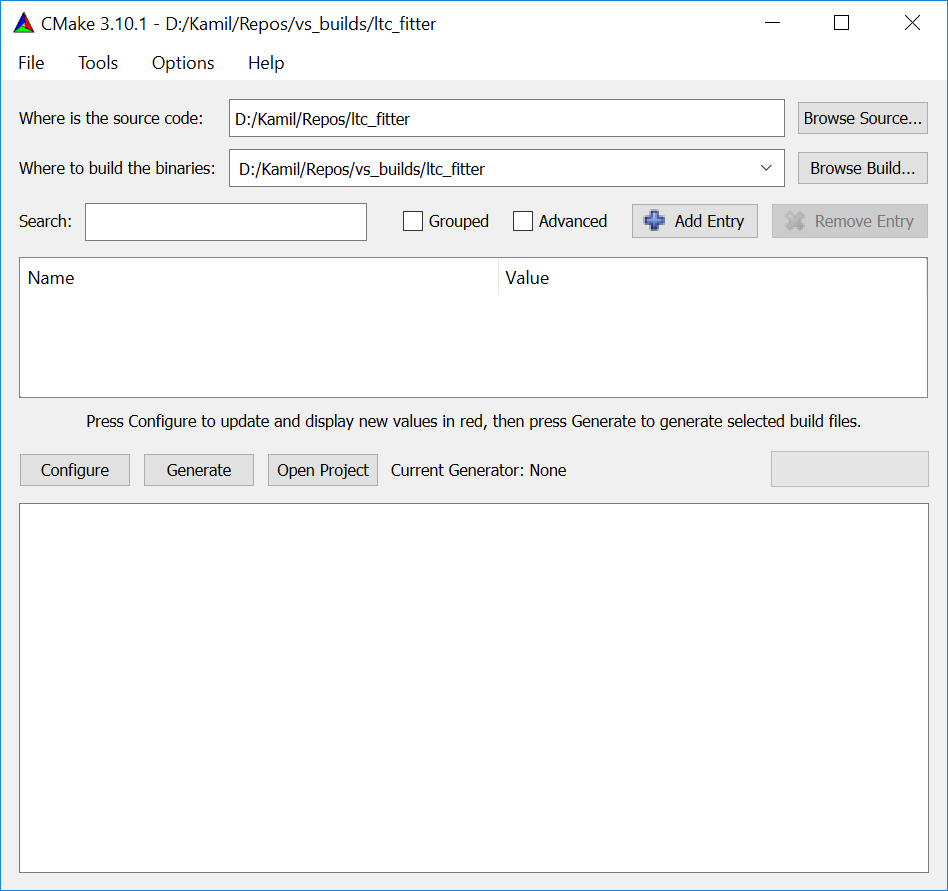
\includegraphics[width=\textwidth]{architecture/cmake/gui-step-1}
        \caption{Wybieramy katalog główny kodu źródłowego w którym znajduje się plik \texttt{CMakeLists.txt} oraz katalog w którym zostaną umieszczone pliki projektu. Klikamy ,,Configure''.}
    \end{subfigure}
    \hspace{0.5cm}
    \begin{subfigure}[t]{0.40\textwidth}
        \centering
        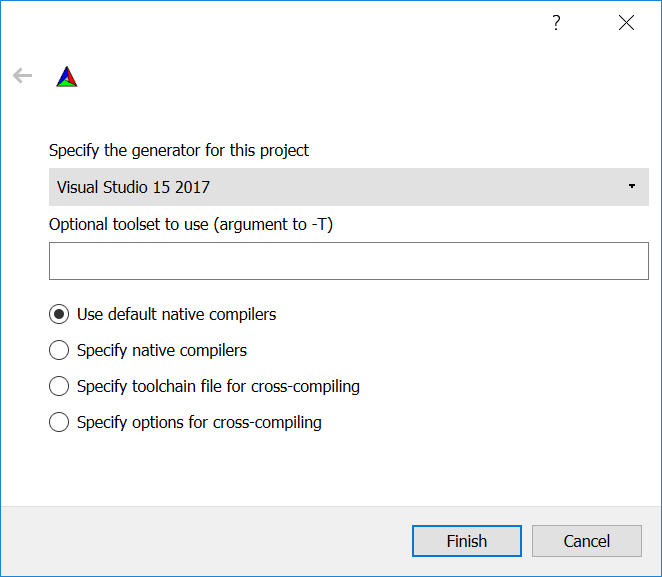
\includegraphics[width=\textwidth]{architecture/cmake/gui-step-2}
        \caption{Wybieramy narzędzie dla którego projekt zostanie wygenerowany, tutaj wybraliśmy ,,Visual Studio 2017''.}
    \end{subfigure}

    \hfill \\ 
    \vspace{0.5cm}

    \begin{subfigure}[t]{0.40\textwidth}
        \centering
        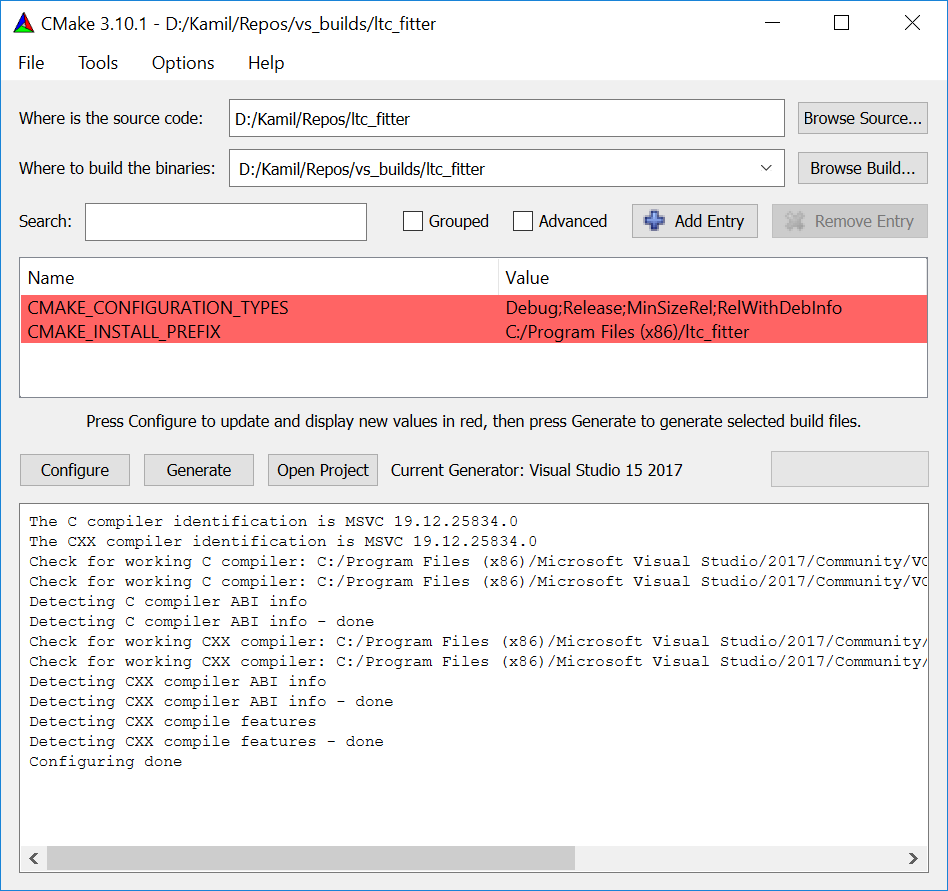
\includegraphics[width=\textwidth]{architecture/cmake/gui-step-3}
        \caption{Po wstępnej konfiguracji pojawiają nam się możliwe opcje do ustawienia, pozostawiamy wszystkie domyślne wartości oraz klikamy ponownie ,,Configure'', następnie ,,Generate''}
    \end{subfigure}
    \hspace{0.5cm}
    \begin{subfigure}[t]{0.40\textwidth}
        \centering
        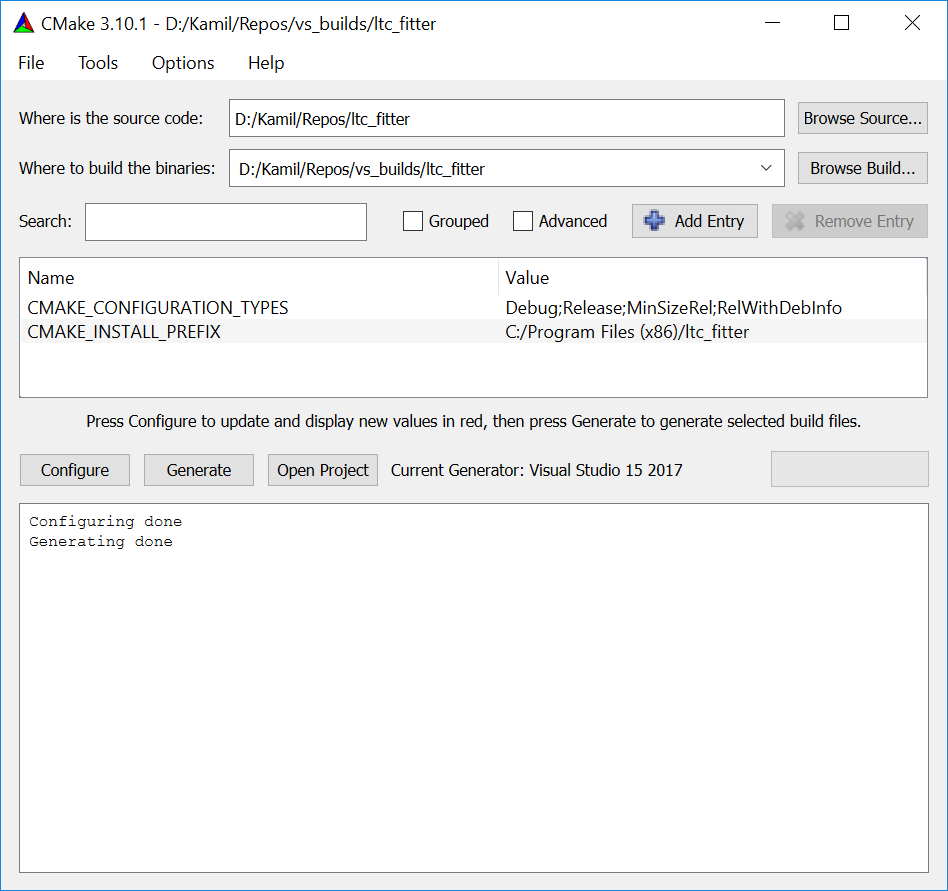
\includegraphics[width=\textwidth]{architecture/cmake/gui-step-4}
        \caption{Projekt został wygenerowany. Po przyciśnięciu ,,Open Project'' powinno otworzyć się IDE w którym możemy skompilować projekt.}
    \end{subfigure}
    
    \caption{Generowanie projektu przy użyciu CMake GUI 3.10.1. Opracowanie własne.}
    \label{fig:CMakeGUIUsage}
\end{figure}


\subsection{Struktura kodu źródłowego}

W główym katalogu repozytorium znajdziemy poszczególne pliki oraz katalogi zawierające wszystko co jest potrzebne do uruchomienia 

\begin{description}
    \item[\texttt{CMakeLists.txt}] \hfill\\ 
    plik opisujący sposób generowania projektów dla poszczególnych IDE 
    
    \item[\texttt{README.md}] \hfill\\ 
    krótki opis aplikacji i podstawowy sposób użytkowania 
    
    \item[\texttt{scripts/}] \hfill\\ 
    skrypty pomocnicze do generowania podglądów i szukania błędów
    
    \item[\texttt{src/}] \hfill\\ 
    katalog ze źródłami aplikacji
    
    \item[\texttt{dependencies/}] \hfill\\ 
    katalog ze źródłami zależności aplikacji, znajdują się tam źródła biblioteki \texttt{glm} \cite{GLMProject} do operacji na wektorach oraz \texttt{stb} \cite{STBProject} do operacji na mapach bitowych
\end{description}

\noindent W katalogu \texttt{src/} znajdziemy kilka katalogów oraz plików z całą funkcjonalnością aplikacji podzielone ze względu na zastosowanie:

\begin{description}
   
    \item[\texttt{brdf/}] \hfill\\
    definicje BRDF, klasy wewnątrz implementują modele wyznaczające wartość $f_r$ dla danego zbioru parametrów: chropowatości $\alpha$, kierunku obserwacji $\omega_o$ oraz kierunku padania światła $\omega_i$
    
    \item[\texttt{exporters/}] \hfill\\
    klasy transformujące dane z postaci używanej wewnątrz aplikacji do formy optymalnej do przekazania do zapisu przez klasy z katalogu \texttt{files/}
    
    \item[\texttt{files/}] \hfill\\ 
    funkcjonalność wejścia-wyjścia, klasy wewnątrz potrafią wczytywać oraz zapisywać pliki podglądu na niskim poziomie
    
    \item[\texttt{fitting/}] \hfill\\
    zbiór klas organizujących dopasowywanie rozkładu lambertowskiego do danego rozkładu opisanego przez BRDF dla danych parametrów
    
    \item[\texttt{ltc/}] \hfill\\
    klasy pozwalające na przeprowadzanie obliczeń na przekształconych liniowo rozkładach kosinusowych, zawiera także funkcjonalność obliczania błędu między rozkładem LTC, a BRDF
     
    \item[\texttt{numerical/}] \hfill\\
    funkcje numeryczne ogólnego zastosowania: metoda pełzającego sympleksu dla dowolnego wymiaru, generowanie losowych próbek, podstawowe estymatory z funkcją błędu dla ograniczeń
    
    \item[\texttt{plotting/}] \hfill\\
    funkcje generujące podgląd dla BRDF i LTC dla danych parametrów, generowanie podglądów pozwala na szybszą analizę dokładności i naprawianie błędów implementacyjnych
    
    \item[\texttt{tests/}] \hfill\\
    katalog z bardzo prostymi testami dymnymi oraz eksporterem podglądów dla wyników otrzymanych przez \cite{ltc_heitz} 
    
    \item[\texttt{utils/}] \hfill\\
    stałe i funkcje, które nie wpasowały się do pozostałych modułów
\end{description}

\subsection{Architektura aplikacji}

Sercem programu jest elastyczna implementacja algorytmu pełzającego sympleksu z możliwością uruchomienia go w wariancie z funkcją kary. Diagram klas zawierający kluczowe elementy do zrozumienia architektury dopasowywania funkcji znajduje się na rys. \ref{fig:FunctionSolveClassDiagram}. Znalezienie parametrów opowiadającym minimum dla danej funkcji wymaga implementacji interfejsu \texttt{error\_estimator}, klasa ta wyznacza wartość błędu dla danych parametrów. Błąd ten minimalizowany jest w trakcie poszukiwania rozwiązania optymalnego. W przypadku funkcji kary, istnieje konieczność wyznaczenia wartości ograniczeń, które potem są przeliczane na dodatkowy, karny błąd zastosowany przez estymator \texttt{penalty\_error\_estimator}. 

\begin{figure}[h]
    \centering
    
\includegraphics[scale=\graphvizscale]{architecture/ltcfitter/fitting.pdf}
    \caption{Wybrane elementy klas dotyczących procesu optymalizacji funkcji. Opracowanie własne.}
    \label{fig:FunctionSolveClassDiagram}
\end{figure}

W celu wykonania obliczeń koniecznych do znalezienia macierzy $M$ transformującej rozkład kosinusowy do postaci bliskiej rozkładowi referencyjnemu musimy dodać kilka elementów do powyższej struktury. Dzięki interfejsom, dodanie rozszerzeń jest bardzo proste. Pierwszym krokiem, jest implementacja BRDF referencyjnego, w naszym przypadku GGX (rys. \ref{fig:BRDFClassDiagram}).

\begin{figure}[h]
    \centering
    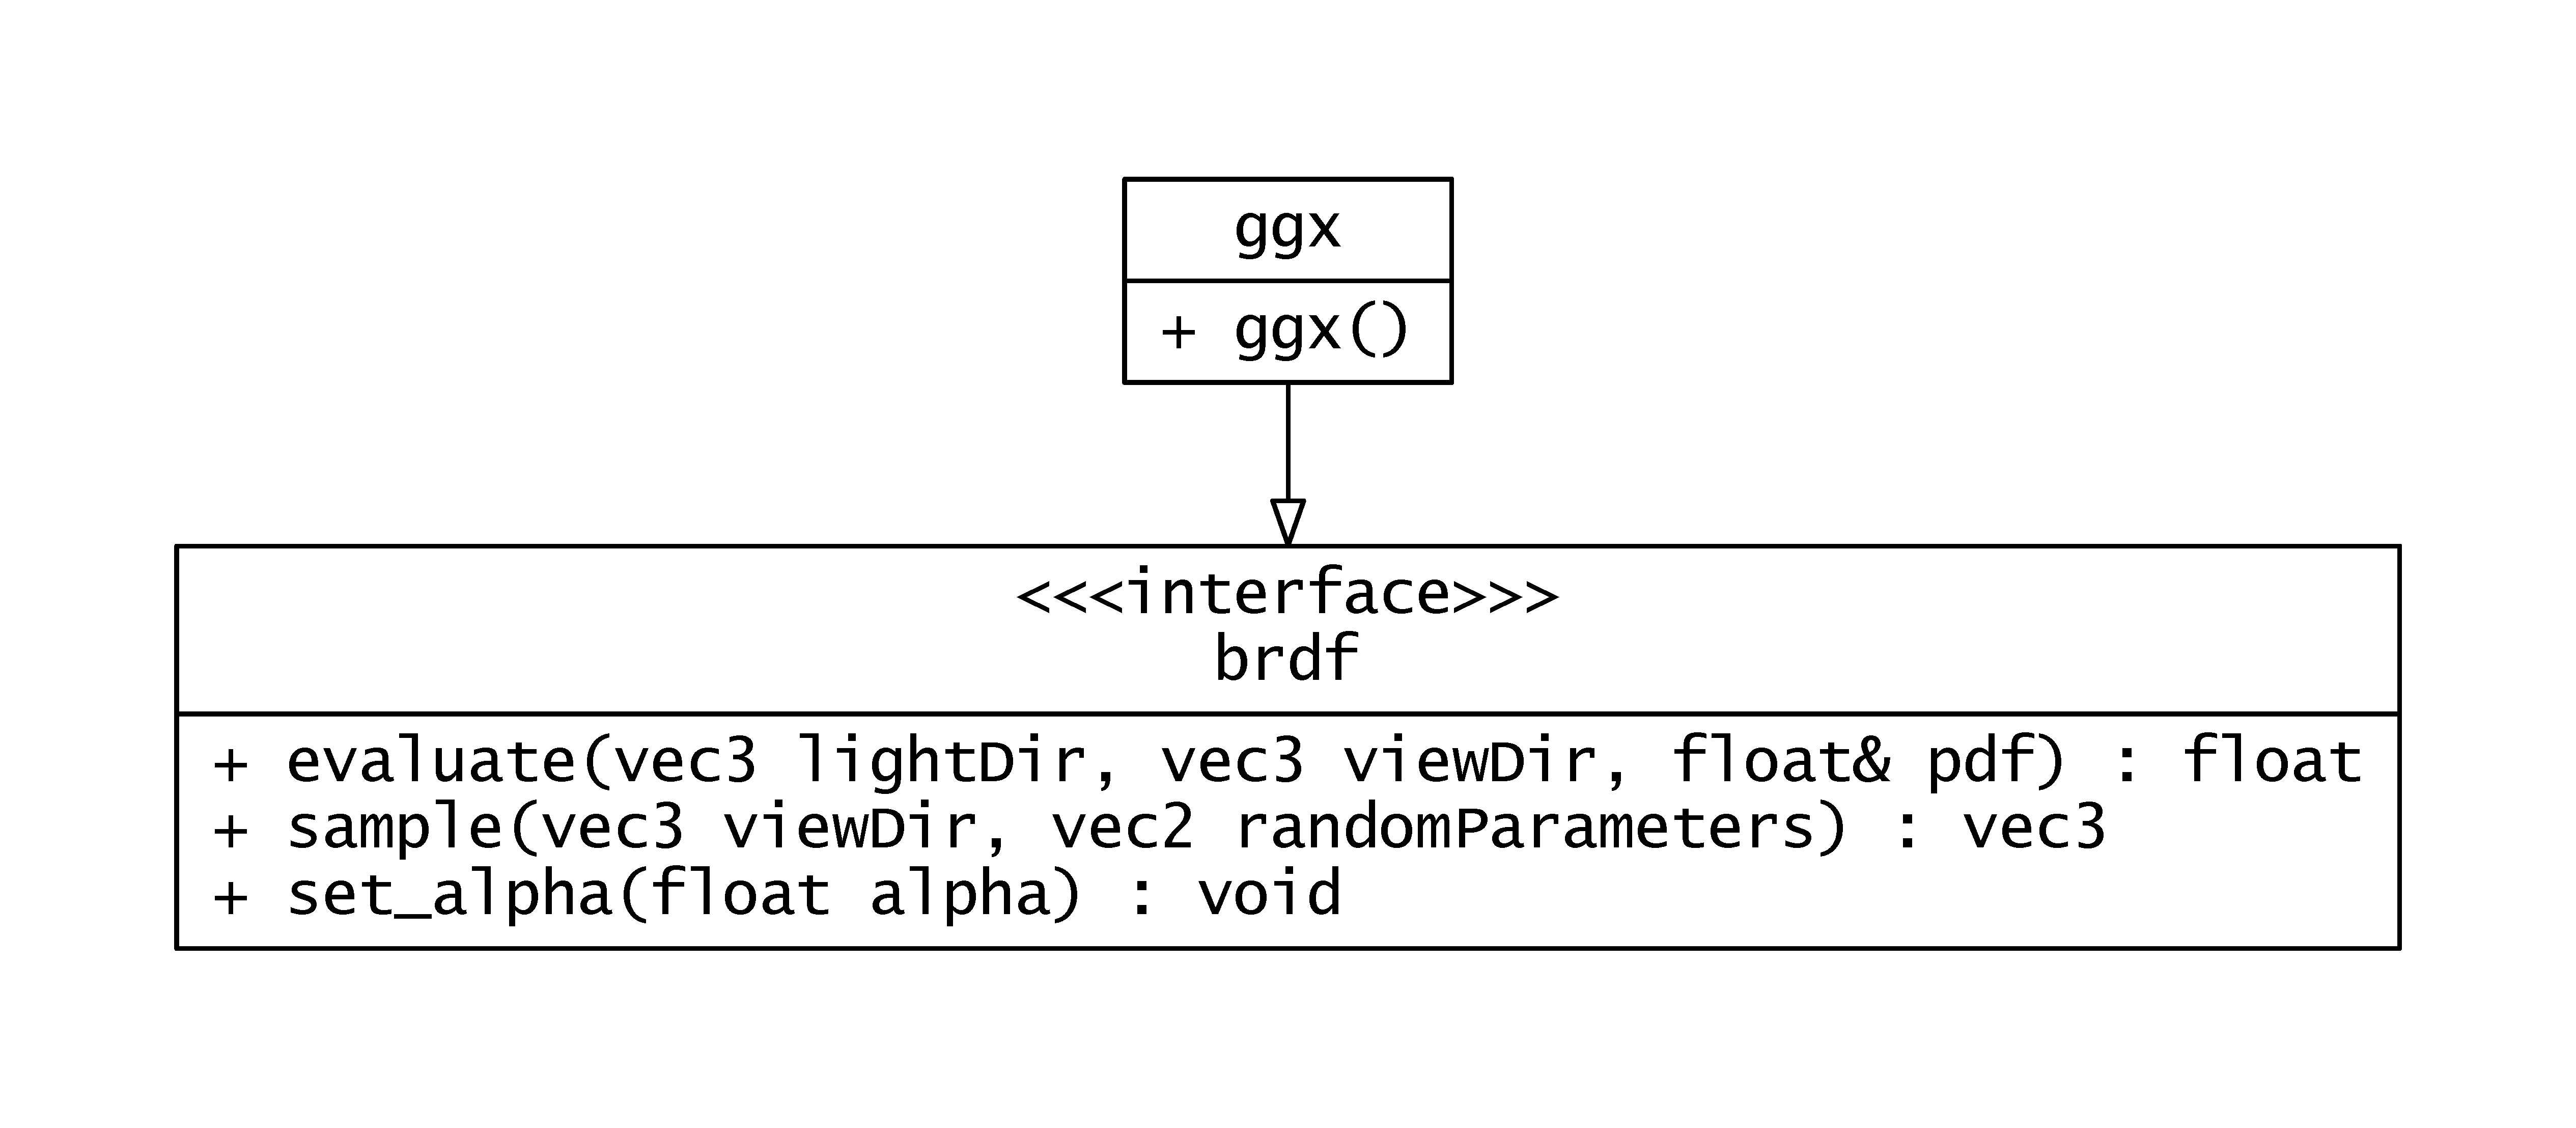
\includegraphics[scale=\graphvizscale]{architecture/ltcfitter/brdf.pdf}
    \caption{Interfejs \texttt{brdf} standaryzujący operacje na modelach BRDF. Opracowanie własne.}
    \label{fig:BRDFClassDiagram}
\end{figure}

Kolejnym krokiem jest implementacja kolejno: 
\begin{enumerate}
    \item reprezentacji liniowo transformowanych kosinusów, którą będziemy traktować jak BRDF,
    \item estymator błędu między obecnym przybliżeniem, a BRDF referencyjnym,
    \item kalkulator ograniczeń, które zostaną wykorzystane do nałożenia kary w przypadku zbliżenia się do granic.
\end{enumerate}

Implementacja już istniejących interfejsów (rys. \ref{fig:LTCClassDiagram}) pozwoli nam na wykorzystanie w pełni mechanizmu wyszukiwania minimum funkcji do znalezienia optymalnej transformacji.

\begin{figure}[h]
    \centering
    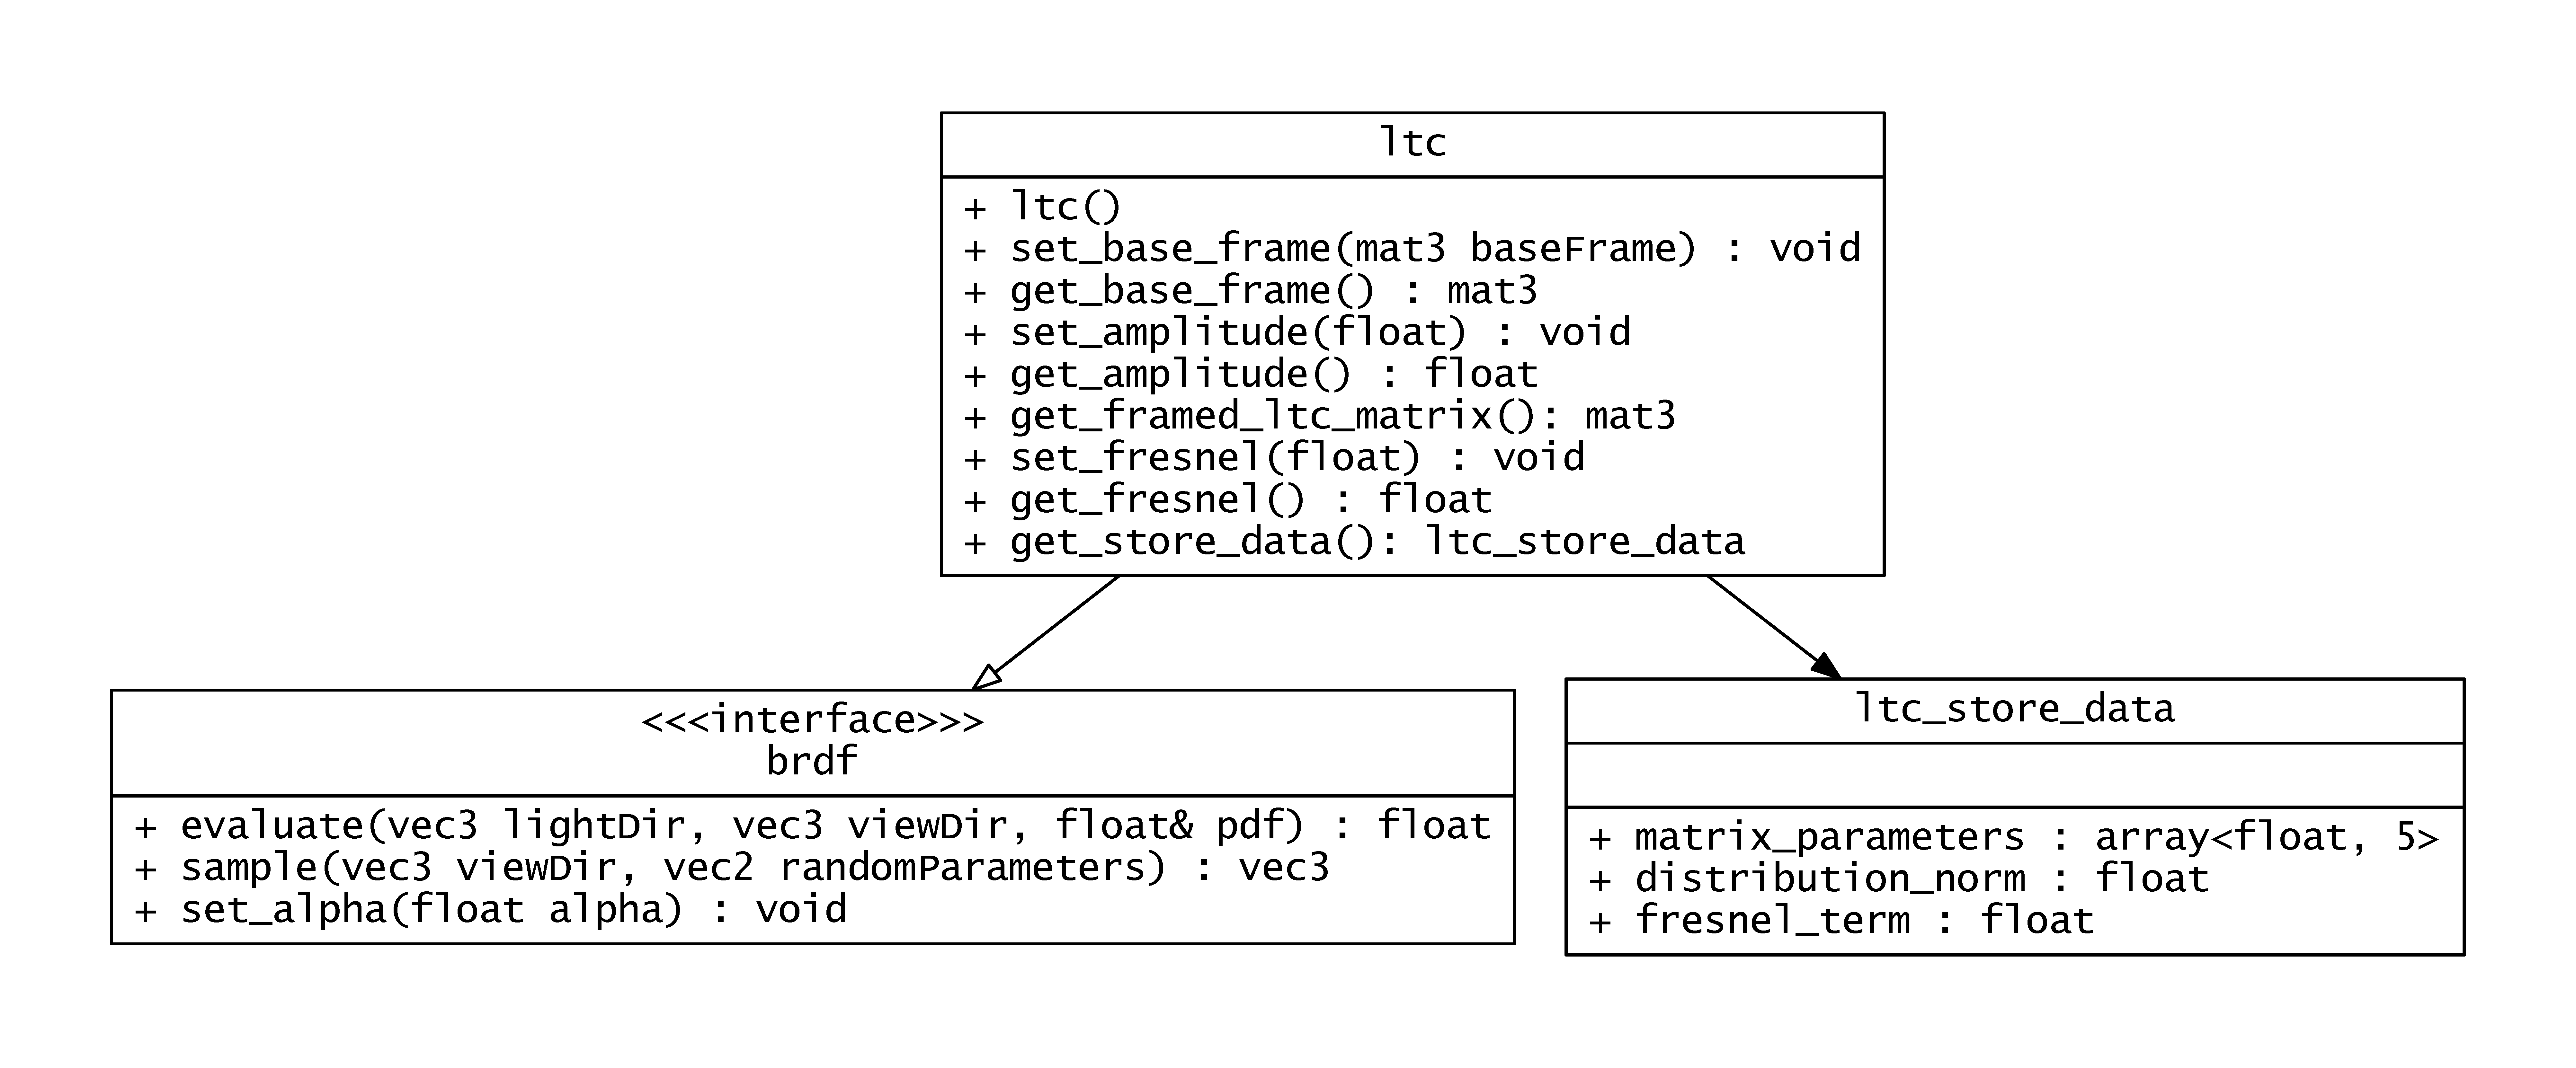
\includegraphics[scale=\graphvizscale]{architecture/ltcfitter/ltc1.pdf}
    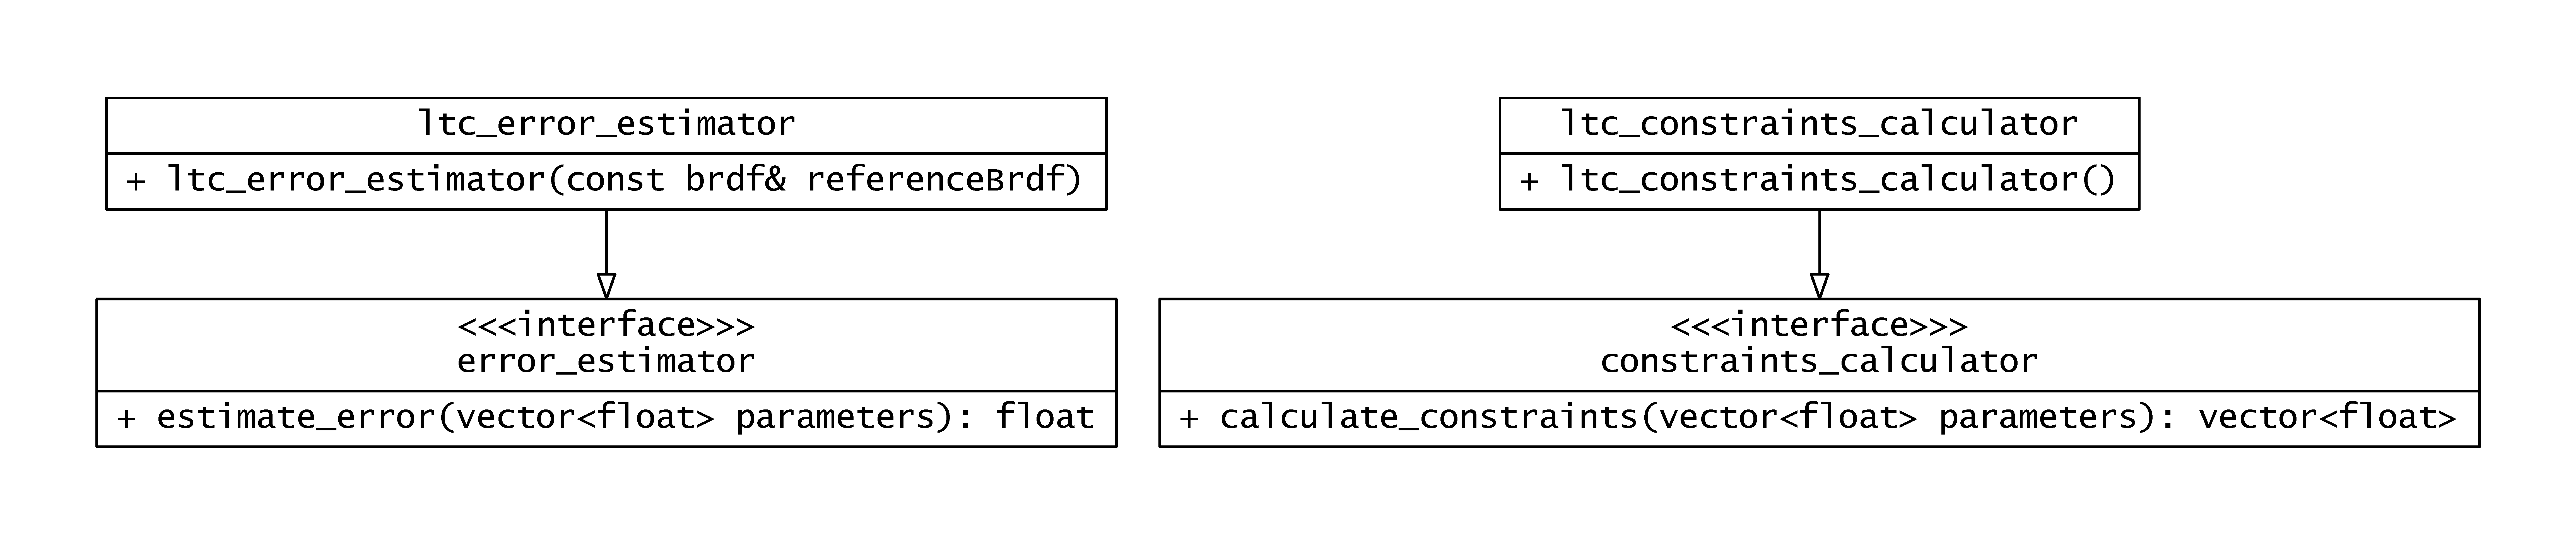
\includegraphics[scale=\graphvizscale]{architecture/ltcfitter/ltc2.pdf}
    \caption{Klasy implementujące wsparcie dla optymalizacji macierzy $M$ dla metody LTC. Opracowanie własne.}
    \label{fig:LTCClassDiagram}
\end{figure}

Procedurę wyznaczania parametrów wejściowych dla BRDF referencyjnego oraz ich zapisu do pliku możemy znaleźć w funkcji \texttt{build\_lookup}. Funkcja ta, dzieli dziedzinę na zadaną liczbę próbek, znajduje przybliżone rozwiązanie początkowe i uruchamia funkcję \texttt{ltc\_fit}, która z kolei buduje drzewo zależności wymagane przez algorytm pływającego sympleksu i znajduje optymalne rozwiązanie dla danych parametrów wejściowych.

\subsection{Możliwe rozszerzenia}

Aplikacja może z łatwością zostać rozszerzona o dodatkowe modele BRDF.

Architektura i specyfika obliczeń sprawia, że obliczenia mogłyby zostać zrównoleglone. W przypadku procesora koszt czasowy powinien być minimalny. Być może warto rozważyć implementację podobnego algorytmu z wykorzystaniem GPU.

\section{Program \texttt{arealights}}

Program \texttt{arealights} jest aplikacją graficzną realizującą algorytmy symulujące światła powierzchniowe zamieszczone w tej pracy.

Kod programu można znaleźć na dołączonej płycie CD lub w repozytorium online pod adresem: \url{https://github.com/sienkiewiczkm/arealights}.

\subsection{Opis użytkowania}

\subsection{Kompilacja}

Kompilacja tego projektu przebiega analogiczne do poprzedniego programu. Szczegóły dotyczące budowania aplikacji można znaleźć w rozdziale \ref{section:ltcFitterCompilation}.

\subsection{Struktura kodu źródłowego}
\subsection{Architektura aplikacji}
\subsection{Możliwe rozszerzenia}

\begin{itemize}
    \item kolorowe światła LTC
    \item inne metody?
\end{itemize}

\end{document}